
The 2D templates are constructed using The \mll~and \mt~ variables.
These variables are defined as follows:

%
\begin{itemize}
\item the dilepton mass $\mll$;
\item transverse Higgs mass, 
$\mt^{\ell\ell\met} = \sqrt{2\pt^{ll}\met(1-cos(\Delta\phi_{\ell\ell-\met}))}$ where 
$\Delta\phi_{\ell\ell-\met}$ is the angle between dilepton
direction and \met in the transverse plane.
\end{itemize} 

Example templates are shown in 
Figure~\ref{fig:templates_125_ex} 
for the Higgs boson signal with a mass \mHi = 125 \GeV~(left) and 
the dominant \qqww~background (right). As expected, the 
\qqww~background peaks at higher values of \mll~than the signal.

%
\begin{figure}[!hbtp]
	
	%
	\centering
	\subfigure[Signal]{
	\centering
	\label{subfig:template_signal_125}
		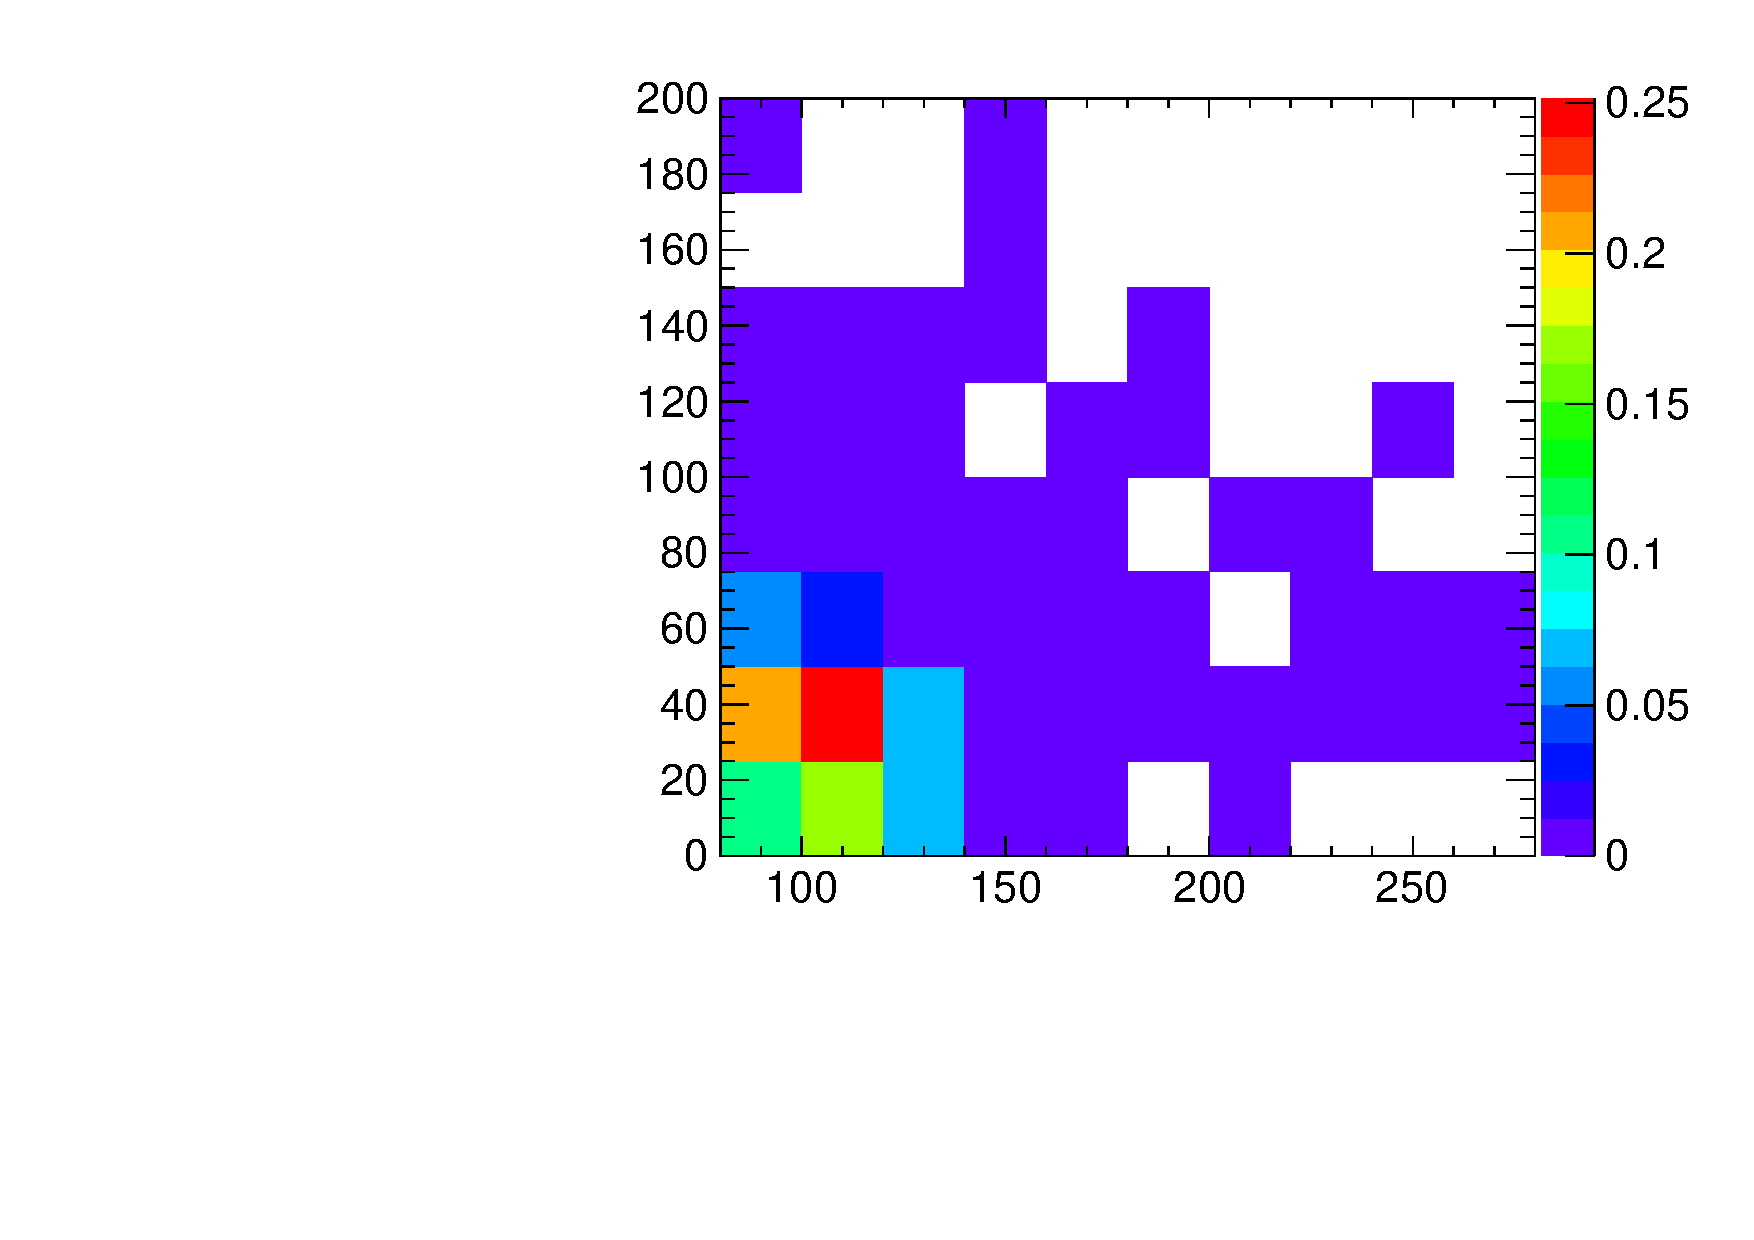
\includegraphics[width=.35\textwidth]{figures/templates/sig_2D_mH125_0j_of.pdf}
	}
	\subfigure[\qqww]{
	\centering
	\label{subfig:template_qqWW_125}
		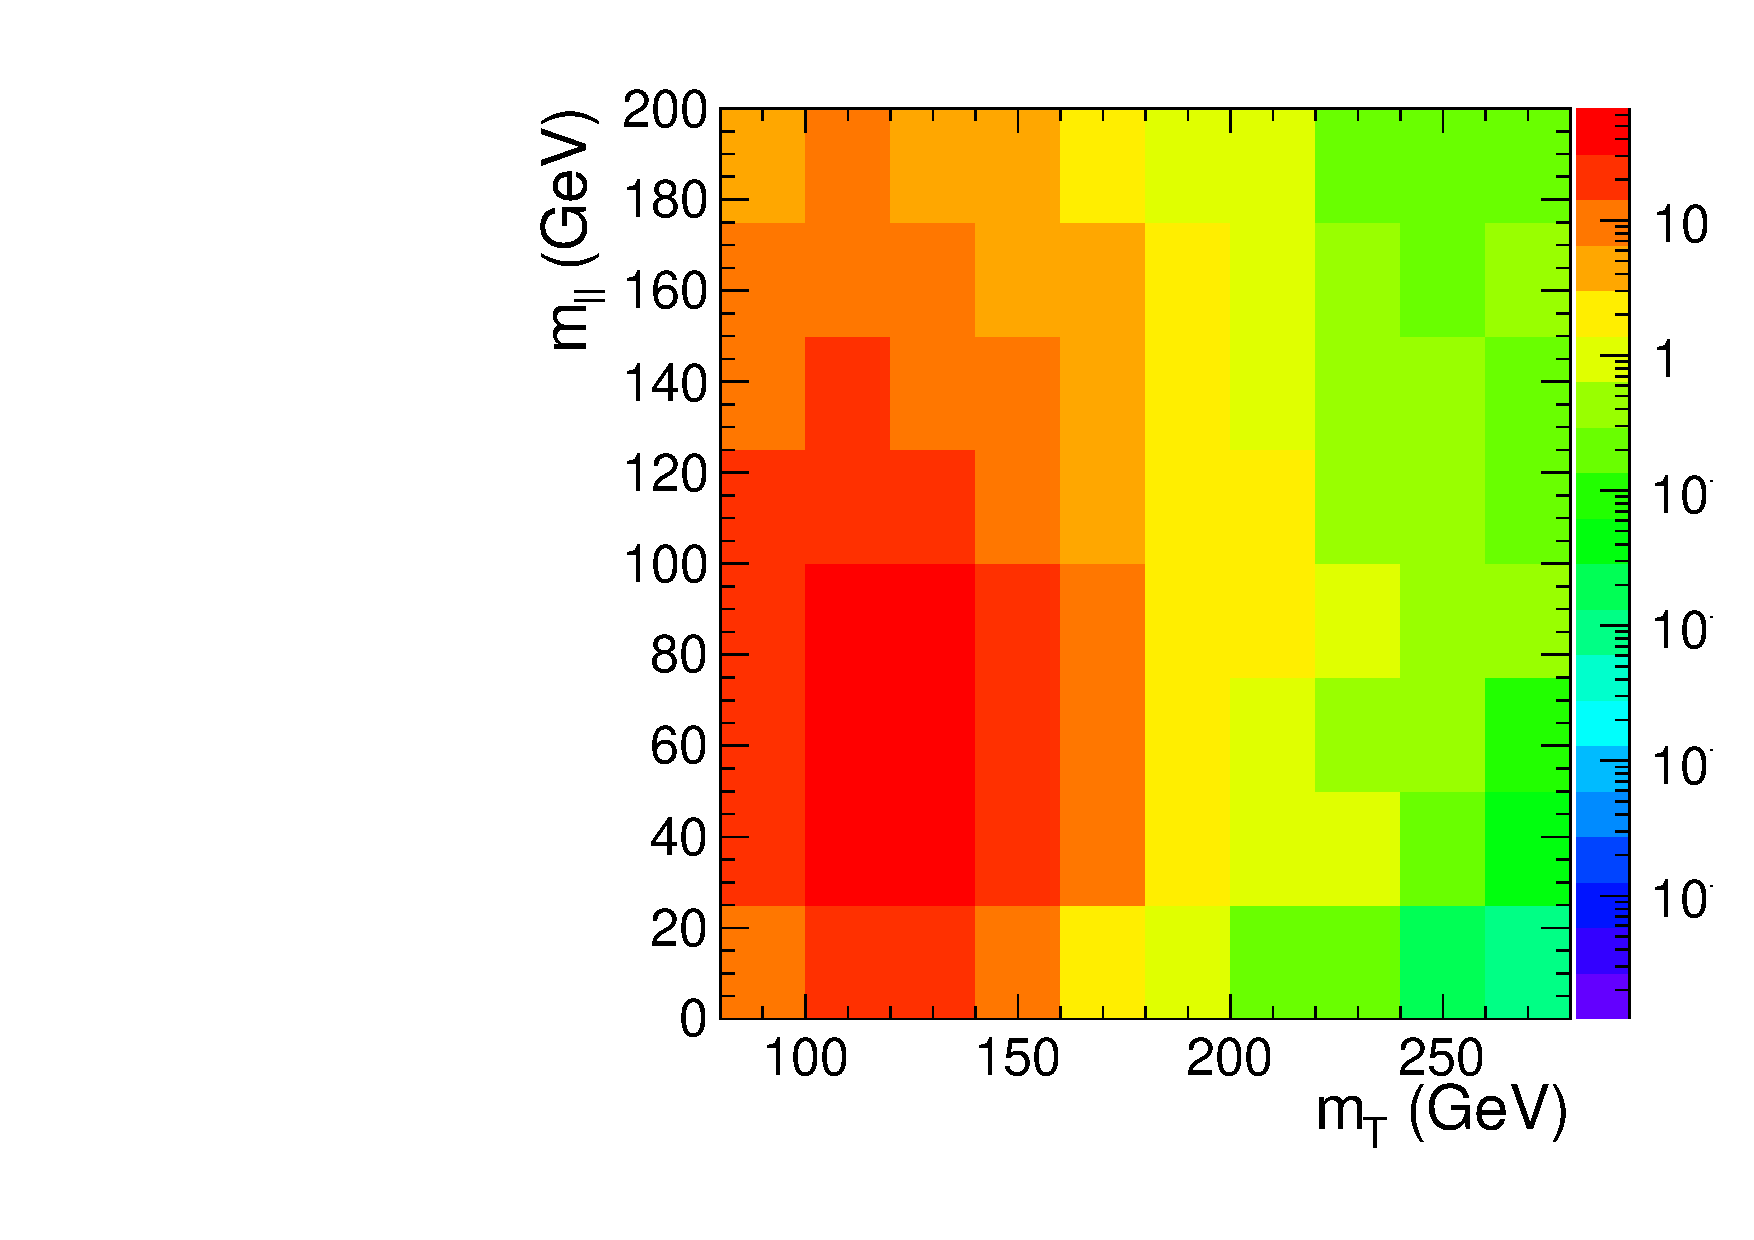
\includegraphics[width=.35\textwidth]{figures/templates/qqWW_2D_mH125_0j_of.pdf}
	}
	
	\caption{2D templates for signal at \mHi = 125 \GeV (left) 
and \qqww~background (right).} 
	\label{fig:templates_125_ex}

\end{figure}
	
